
%\documentclass[mathserif]{beamer}
\documentclass[handout]{beamer}
%\usetheme{Goettingen}
%\usetheme{Warsaw}
\usetheme{Singapore}



%\usetheme{Frankfurt}
%\usetheme{Copenhagen}
%\usetheme{Szeged}
%\usetheme{Montpellier}
%\usetheme{CambridgeUS}
%\usecolortheme{}
%\setbeamercovered{transparent}
\usepackage[english, activeacute]{babel}
\usepackage[utf8]{inputenc}
\usepackage{amsmath, amssymb}
\usepackage{dsfont}
\usepackage{graphics}
\usepackage{cases}
\usepackage{graphicx}
\usepackage{pgf}
\usepackage{epsfig}
\usepackage{amssymb}
\usepackage{multirow}	
\usepackage{amstext}
\usepackage[ruled,vlined,lined]{algorithm2e}
\usepackage{amsmath}
\usepackage{epic}
\usepackage{epsfig}
\usepackage{fontenc}
\usepackage{framed,color}
\usepackage{palatino, url, multicol}
%\algsetup{indent=2em}
\newcommand{\factorial}{\ensuremath{\mbox{\sc Factorial}}}
\newcommand{\BIGOP}[1]{\mathop{\mathchoice%
{\raise-0.22em\hbox{\huge $#1$}}%
{\raise-0.05em\hbox{\Large $#1$}}{\hbox{\large $#1$}}{#1}}}
\newcommand{\bigtimes}{\BIGOP{\times}}
\vspace{-0.5cm}
\title{Natural Language Processing \\ Transformer Architecture}
\vspace{-0.5cm}
\author[Felipe Bravo Márquez]{\footnotesize
%\author{\footnotesize  
 \textcolor[rgb]{0.00,0.00,1.00}{Felipe Bravo-Marquez}} 
  
 

\date{\today}

\begin{document}
\begin{frame}
\titlepage


\end{frame}



\begin{frame}{What's Wrong with RNNs?}
\begin{scriptsize}
\begin{itemize}
\item Given what we just learned on previous lecture, it would seem like attention solves all the problems with RNNs and encoder-decoder architectures\footnote{The following material is based on: \url{http://mlexplained.com/2017/12/29/attention-is-all-you-need-explained/} and \url{http://jalammar.github.io/illustrated-transformer/}}.

\item There are a few shortcomings of RNNs that another architecture called the \textbf{Transformer} tries to address.

\item The Transformer discards the recursive component of the Encoder-Decoder architecture and purely relies on attention mechanisms \cite{vaswani2017attention}.

\item When we process a sequence using RNNs, each hidden state depends on the previous hidden state. 

\item This becomes a major pain point on GPUs: GPUs have a lot of computational capability and they hate having to wait for data to become available.

\item Even with technologies like CuDNN, RNNs are painfully inefficient and slow on the GPU.


\end{itemize}
\end{scriptsize}
\end{frame}

\begin{frame}{Dependencies in neural machine translations}
\begin{scriptsize}
In essence, there are three kinds of dependencies in neural machine translations: 
\begin{enumerate}
\item Dependencies between the input and output tokens.

\item Dependencies between the input tokens themselves.

\item Dependencies between the output tokens themselves.
\end{enumerate}


The traditional attention mechanism largely solved the first dependency by giving the decoder access to the entire input sequence. The second and third dependencies were addressed by the RNNs.

\end{scriptsize}

\end{frame}


\begin{frame}{The Transformer}
\begin{scriptsize}
\begin{itemize}
 \item The novel idea of the Transformer is to extend this mechanism to the processing input and output sentences as well.
 \item The RNN processes input sequences sequentially. 
 \item The Transformer, on the other hand, allows the encoder and decoder to see the entire input sequence all at once.
 \item This is done using attention.
\end{itemize}



\end{scriptsize}

\end{frame}



\begin{frame}{The Transformer}
\begin{scriptsize}
 \begin{itemize}
  \item Let’s begin by looking at the Transformer as a single black box. 
  \item In a machine translation application, it would take a sentence in one language, and output its translation in another.
 \end{itemize}

\end{scriptsize}



     \begin{figure}[h]
        	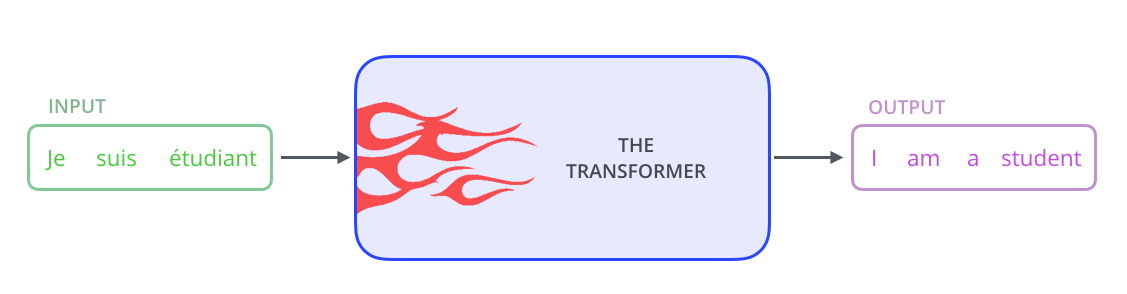
\includegraphics[scale = 0.29]{pics/the_transformer_3.png}
        \end{figure}  


\end{frame}


\begin{frame}{The Transformer}
\begin{scriptsize}
 \begin{itemize}
  \item  This blackbox can be decomposed by an encoding component, a decoding component, and connections between them.
 \end{itemize}

\end{scriptsize}



     \begin{figure}[h]
        	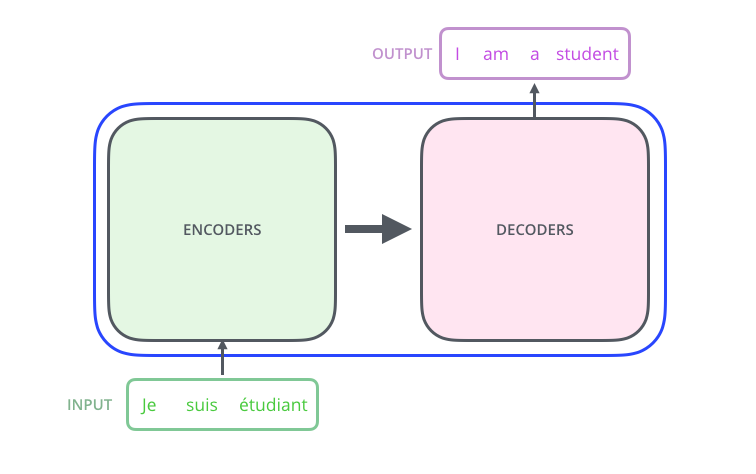
\includegraphics[scale = 0.29]{pics/The_transformer_encoders_decoders.png}
        \end{figure}  


\end{frame}

\begin{frame}{The Transformer}
\begin{scriptsize}
 \begin{itemize}
  \item  The encoding component is a stack of encoders.
  \item The original Transformer stacks six of them on top of each other.
  \item But there’s nothing magical about the number six, one can definitely experiment with other arrangements. 
  \item The decoding component is a stack of decoders of the same number.
 \end{itemize}

\end{scriptsize}



     \begin{figure}[h]
        	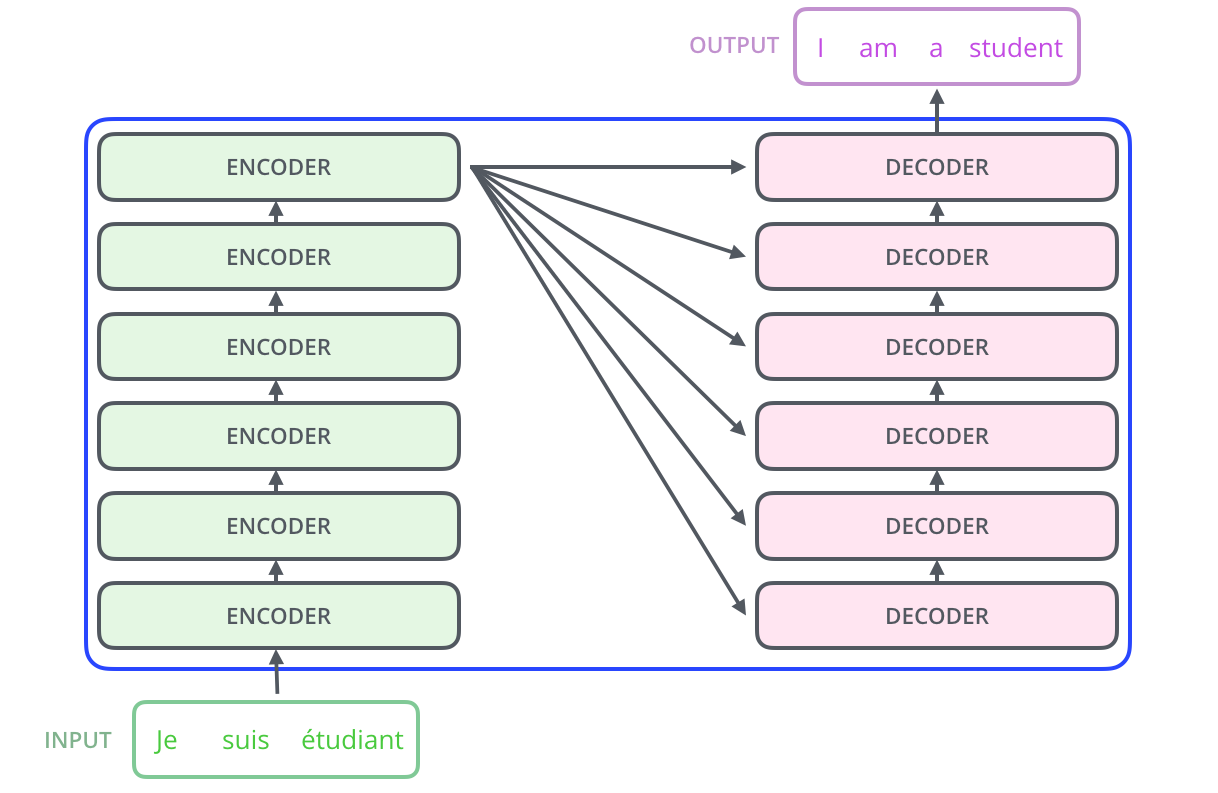
\includegraphics[scale = 0.2]{pics/The_transformer_encoder_decoder_stack.png}
        \end{figure}  


\end{frame}


\begin{frame}{The Transformer}

     \begin{figure}[h]
        	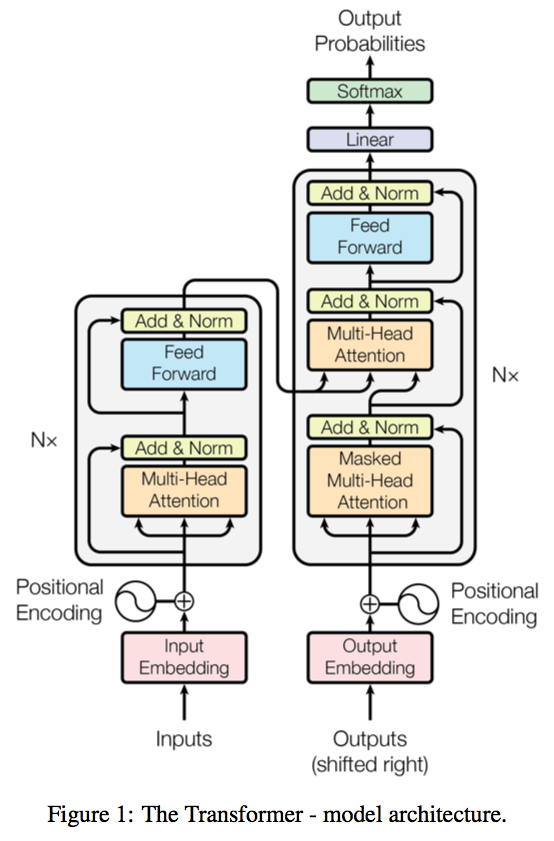
\includegraphics[scale = 0.29]{pics/transformer.png}
        \end{figure}  


\end{frame}


\begin{frame}{The Transformer}
\begin{scriptsize}
\begin{itemize}

 \item  The Transformer still uses the basic encoder-decoder design of RNN neural machine translation systems.
 
 \item The left-hand side is the encoder, and the right-hand side is the decoder. 
 
 \item The initial inputs to the encoder are the embeddings of the input sequence.
 \item The initial inputs to the decoder are the embeddings of the outputs up to that point. 
 
 \item The encoder and decoder are composed of $N$ blocks (where $N = 6$ for both networks).
 
 \item These blocks are composed of smaller blocks as well. 
 
 \item Before looking at each block in further detail, let't try to understand the Attention mechanism implemented by the Transformer.
 
\end{itemize}

\end{scriptsize}

\end{frame}




\begin{frame}{Attention Mechanism in the Transformer}
\begin{scriptsize}
\begin{itemize}
 \item The attention mechanism in the Transformer is interpreted as a way of computing the relevance of a set of \textbf{values} (information) based on some \textbf{keys} and \textbf{queries}. 
 
 \item The attention mechanism is used as a way for the model to \textbf{focus on relevant information} based on what it is currently processing.
 
 \item In the RNN encoder-decoder architecture with attention:
 

 \begin{enumerate}
  \begin{scriptsize}
 \item Attention weights were the relevance of the encoder hidden states (values) in processing the decoder state (query).
 
 \item These values were calculated based on the encoder hidden states (keys) and the decoder hidden state (query).
 \end{scriptsize}

 \end{enumerate}

 
\end{itemize}



\end{scriptsize}

\end{frame}



\begin{frame}{Attention Mechanism in the Transformer}

    \begin{figure}[h]
        	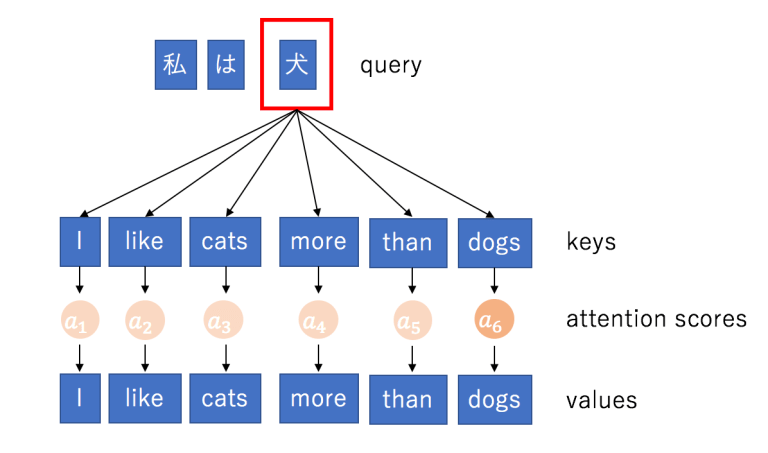
\includegraphics[scale = 0.2]{pics/attention_concept.png}
        \end{figure}  

\begin{scriptsize}
\begin{itemize}        
\item In this example, the query is the word being decoded (which means dog) and both the keys and values are the source sentence. 
\item The attention score represents the relevance, and in this case is large for the word “dog” and small for others.
 \item When we think of attention this way, we can see that the keys, values, and queries could be anything. 
 \item They could even be the same. 
 \item For instance, both values and queries could be input embeddings (self attention). 
\end{itemize}

\end{scriptsize}

\end{frame}


\begin{frame}{Queries}



\begin{scriptsize}
\begin{itemize}
\item Queries are representations of the target or output sequence that the Transformer model uses to determine how much attention should be given to each word in the input sequence.
\item Each word or token in the output sequence is associated with a query.
\item The queries help in retrieving relevant information from the input sequence.
\item Example: If we are generating the translation for the sentence ``Je adore les chats'' (meaning "I love cats" in French), each word in the output sequence would have its corresponding query representation.
\item For example, ``Je'' would have a query vector, ``adore'' would have a query vector, and so on.


\end{itemize}

\end{scriptsize}

\end{frame}


\begin{frame}{Keys}



\begin{scriptsize}
\begin{itemize}
\item Keys are representations of the input sequence that the Transformer model uses to compute the attention scores.
\item Each word or token in the input sequence is associated with a key.
\item These keys capture the information needed to understand the context and relationships between words in the sequence.
\item Example: Consider the input sequence: ``I love cats.''
\item Each word in the sequence would have its corresponding key representation, such as ``I'' having a key vector, ``love'' having a key vector, and so on.

\end{itemize}

\end{scriptsize}

\end{frame}





\begin{frame}{Values}



\begin{scriptsize}
\begin{itemize}
\item Values are the actual information or features associated with each word in the input sequence.
\item These values are used to calculate the weighted sum during the attention computation, which helps determine the importance or relevance of each word.
\item Example: Considering the same input sequence ``I love cats,'' each word would have its associated value representation.
\item These values contain the contextual information for each word.
\item For instance, ``I'' would have a value vector, ``love'' would have a value vector, and so forth.
\item Keys and values are very difficult to distinguish at first sight because in RNN encoding and decoding with classical attention they are the same.
\item We will see with the Transformer that although they come from the same sequence, they may correspond to different vectors.

\end{itemize}

\end{scriptsize}

\end{frame}


\begin{frame}{Scaled Dot Product Attention}
\begin{scriptsize}
\begin{itemize}

  \item  Transformer uses a particular form of attention called the “Scaled Dot-Product Attention”:

  \item For a given query vector $\vec{q}$, a sequence of key vectors $\vec{k}_{1:m}$, and a sequence of value vectors $\vec{v}_{1:m}$,  the attention weights $\alpha_1,\dots,\alpha_m$  are computed as follows:


  \begin{displaymath}
    \alpha_1,\dots,\alpha_m = \text{softmax}\left(\frac{\vec{q} \cdot \vec{k}_{1}}{\sqrt{d}}, \dots,\frac{\vec{q} \cdot \vec{k}_{1}}{\sqrt{d}}\right)
  \end{displaymath}


 \item $d$ represents the dimensionality of the queries and keys.

  \item The normalization over $\sqrt{d}$ is used to rescale the dot products between queries and keys (dot products tend to grow with the dimensionality).

  \item The attention weights are then multiplied by their corresponding values to compute a weighted sum, which is then passed to the subsequent layers of the network:

  \begin{displaymath}
   \alpha_1*\vec{v}_1+\cdots+\alpha_m*\vec{v}_m
  \end{displaymath}

 \item Now we are ready to take a closer look at each part of the Transformer.


\end{itemize}

\end{scriptsize}

\end{frame}








\begin{frame}{The Encoder}
\begin{scriptsize}
\begin{itemize}

\item The encoder contains self-attention layers. 

\item In a self-attention layer all of the keys, values and queries come from the same place, in this case, the output of the previous layer in the encoder. 

\item Each position in the encoder can attend to all positions in the previous layer of the encoder.

 \item  The encoder is composed of two blocks (which we will call sub-layers to distinguish from the $N$ blocks composing the encoder and decoder).
\item  One is the Multi-Head Attention sub-layer over the inputs, mentioned above. 
\item The other is a simple feed-forward network. 

\end{itemize}

\end{scriptsize}


    


\end{frame}



\begin{frame}{The Encoder}



     \begin{figure}[h]
        	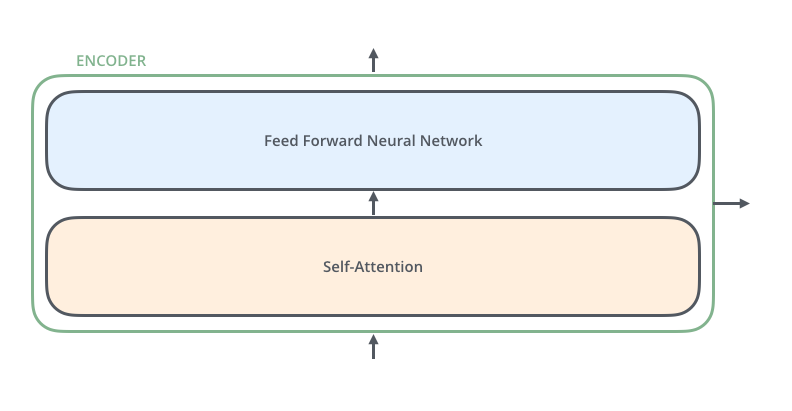
\includegraphics[scale = 0.35]{pics/Transformer_encoder.png}
        \end{figure}  





\end{frame}


\begin{frame}{Bringing The Tensors Into The Picture}
\begin{scriptsize}
\begin{itemize}



\item We begin by turning each input word into a vector using an embedding layer  of the size 512 in the bottom-most encoder.

\begin{figure}[h]
        	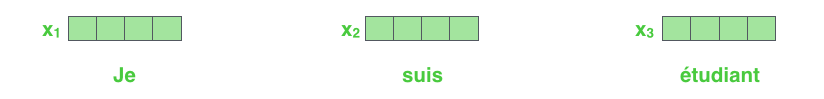
\includegraphics[scale = 0.35]{pics/embeddings_enc.png}
        \end{figure}  




\item In the bottom encoder that would be the word embeddings, but in other encoders, it would be the output of the encoder that's directly below.

\item The size of this list is hyperparameter we can set – basically it would be the length of the longest sentence in our training dataset.


\end{itemize}

\end{scriptsize}

    

\end{frame}





\begin{frame}{Bringing The Tensors Into The Picture}
\begin{scriptsize}

\begin{figure}[h]
        	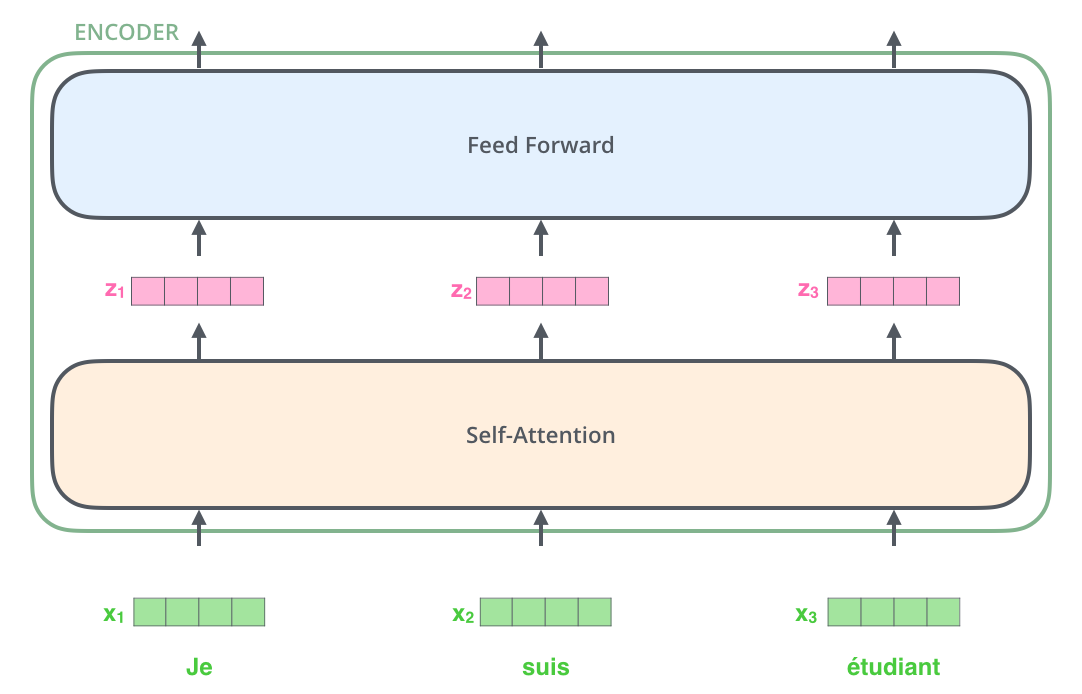
\includegraphics[scale = 0.2]{pics/encoder_with_tensors.png}
        \end{figure}  

\begin{itemize}


\item The word in each position flows through its own path in the encoder. 

\item There are dependencies between these paths in the self-attention layer. 

\item The feed-forward layer does not have those dependencies.

\item However, and thus the various paths can be executed in parallel while flowing through the feed-forward layer.


\end{itemize}

\end{scriptsize}


\end{frame}


\begin{frame}{Now We’re Encoding!}
\begin{scriptsize}


\begin{itemize}


\item As we've mentioned already, an encoder receives a list of vectors as input. 

\item It processes this list by passing these vectors into a 'self-attention' layer, then into a feed-forward neural network, then sends out the output upwards to the next encoder.

\end{itemize}

\begin{figure}[h]
        	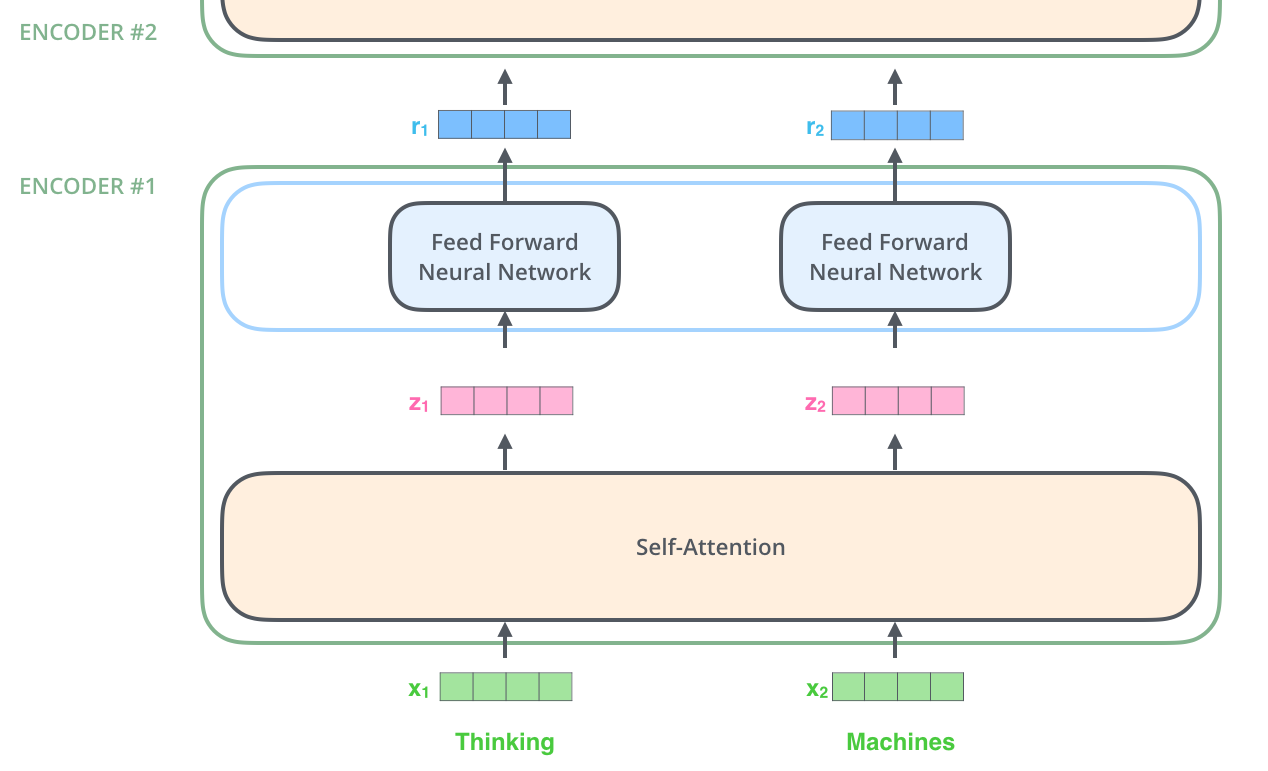
\includegraphics[scale = 0.2]{pics/encoder_with_tensors_2.png}
        \end{figure}  


\end{scriptsize}


\end{frame}


\begin{frame}{Self-Attention at a High Level}
\begin{scriptsize}



\begin{itemize}


\item Say the following sentence is an input sentence we want to translate: 
\\ \textcolor{red}{``The animal didn't cross the street because it was too tired''}

\item What does ``it'' in this sentence refer to? 

\item Is it referring to the street or to the animal? 
\item It's a simple question to a human, but not as simple to an algorithm.

\item When the model is processing the word ``it'', self-attention allows it to associate ``it'' with ``animal''.

\item As the model processes each word (each position in the input sequence), self attention allows it to look at other positions in the input sequence for clues that can help lead to a better encoding for this word.


\end{itemize}

\end{scriptsize}


\end{frame}


\begin{frame}{Self-Attention at a High Level}
\begin{scriptsize}



\begin{itemize}


\item Think of how maintaining a hidden state allows an RNN to incorporate its representation of previous words/vectors it has processed with the current one it's processing. 

\item Self-attention is the method the Transformer uses to bake the ``understanding'' of other relevant words into the one we're currently processing.


\end{itemize}

\end{scriptsize}

\begin{figure}[h]
        	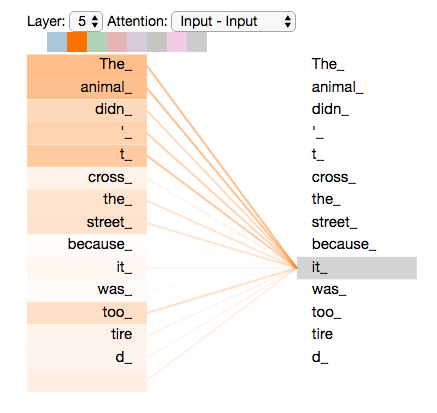
\includegraphics[scale = 0.35]{pics/transformer_self-attention_visualization.png}
        \end{figure}  


\end{frame}



\begin{frame}{Self-Attention in Detail: step 1}
\begin{scriptsize}



\begin{itemize}


\item The \textbf{first step} in calculating scaled dot product self-attention is to create three vectors from each of the encoder's input vectors (in this case, the embedding of each word).

\item So for each word, we create a Query vector, a Key vector, and a Value vector.

\item These vectors are created by multiplying the embedding by three matrices that we trained during the training process.

\item Notice that these new vectors are smaller in dimension than the embedding vector. 

\item Their dimensionality is 64, while the embedding and encoder input/output vectors have dimensionality of 512. 

\item They don’t HAVE to be smaller, this is an architecture choice to make the computation of multiheaded attention (mostly) constant.

\end{itemize}

\end{scriptsize}


\end{frame}



\begin{frame}{Self-Attention in Detail: step 1}


\begin{figure}[h]
        	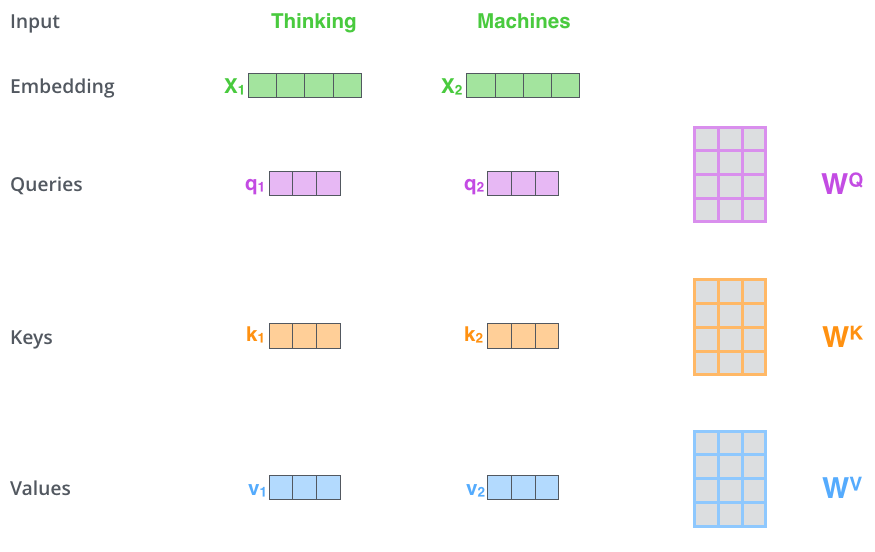
\includegraphics[scale = 0.3]{pics/transformer_self_attention_vectors.png}
        \end{figure}  

\begin{scriptsize}


\begin{itemize}        
\item Example sentence: ``Thinking Machines''.
\item Multiplying \textcolor{green}{$x_1$} by the \textcolor{purple}{WQ} weight matrix produces \textcolor{purple}{$q_1$}, the ``query'' vector associated with that word.
\item We end up creating a ``query'', a ``key'', and a ``value'' projection of each word in the input sentence.

\end{itemize}

\end{scriptsize}


        

\end{frame}


\begin{frame}{Self-Attention in Detail: step 2}
\begin{scriptsize}



\begin{itemize}


\item The \textbf{second step} in calculating self-attention is to calculate a score. 

\item Say we’re calculating the self-attention for the first word in this example, ``Thinking''.

\item We need to score each word of the input sentence against this word. 

\item The score determines how much focus to place on other parts of the input sentence as we encode a word at a certain position.

\item The score is calculated by taking the dot product of the \textcolor{purple}{query vector} with the \textcolor{orange}{key vector} of the respective word we're scoring. 
\item So if we're processing the self-attention for the word in position \textcolor{green}{\#1}, the first score would be the dot product of \textcolor{purple}{q1} and \textcolor{orange}{k1}.
\item The second score would be the dot product of \textcolor{purple}{q1} and \textcolor{orange}{k2}.

\end{itemize}

\end{scriptsize}


\end{frame}


\begin{frame}{Self-Attention in Detail: step 2}


\begin{figure}[h]
        	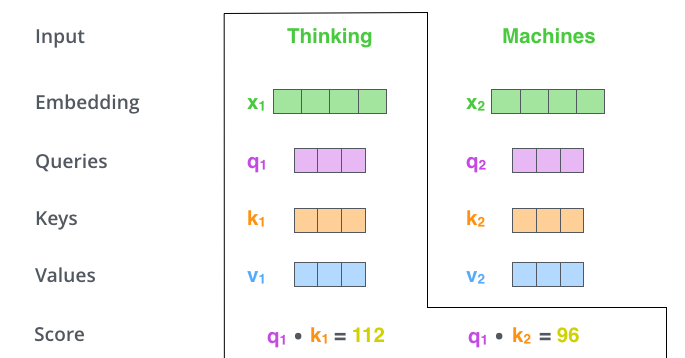
\includegraphics[scale = 0.4]{pics/transformer_self_attention_score.png}
        \end{figure} 




\end{frame}


\begin{frame}{Self-Attention in Detail: steps 3 and 4}
\begin{scriptsize}
\begin{itemize}


\item The \textbf{third} and \textbf{fourth} steps are to divide the scores by 8 (the square root of the dimension of the key vectors used in the paper – 64).

\item This leads to having more stable gradients. 

\item There could be other possible values here, but this is the default), then pass the result through a softmax operation. 

\item Softmax normalizes the scores so they’re all positive and add up to 1.

\item This softmax score determines how much each word will be expressed at the current position. 

\item Clearly the word at the current position will have the highest softmax score, but sometimes it’s useful to attend to another word that is relevant to the current word.

\end{itemize}

\end{scriptsize}


\end{frame}




\begin{frame}{Self-Attention in Detail: steps 3 and 4}


\begin{figure}[h]
        	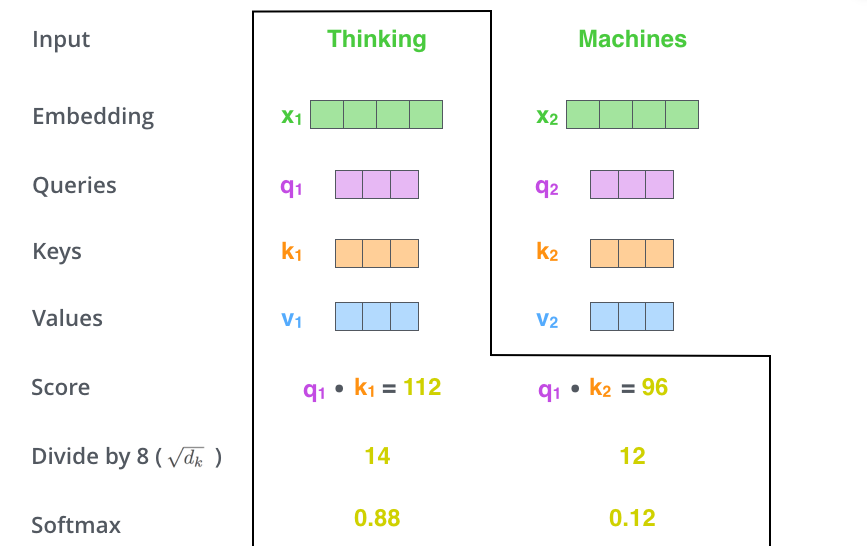
\includegraphics[scale = 0.35]{pics/self-attention_softmax.png}
        \end{figure} 


\end{frame}



\begin{frame}{Self-Attention in Detail: steps 5 and 6}
\begin{scriptsize}
\begin{itemize}


\item The \textbf{fifth step} is to multiply each value vector by the softmax score (in preparation to sum them up).

\item The intuition here is to keep intact the values of the word(s) we want to focus on, and drown-out irrelevant words (by multiplying them by tiny numbers like 0.001, for example).

\item The \textbf{sixth step} is to sum up the weighted value vectors.

\item This produces the output of the self-attention layer at the current position (for the first word in this example).

\item That concludes the scaled dot product self-attention calculation.

\item The resulting vector is one we can send along to the feed-forward neural network.


\end{itemize}

\end{scriptsize}


\end{frame}

\begin{frame}{Self-Attention in Detail: steps 5 and 6}


\begin{figure}[h]
        	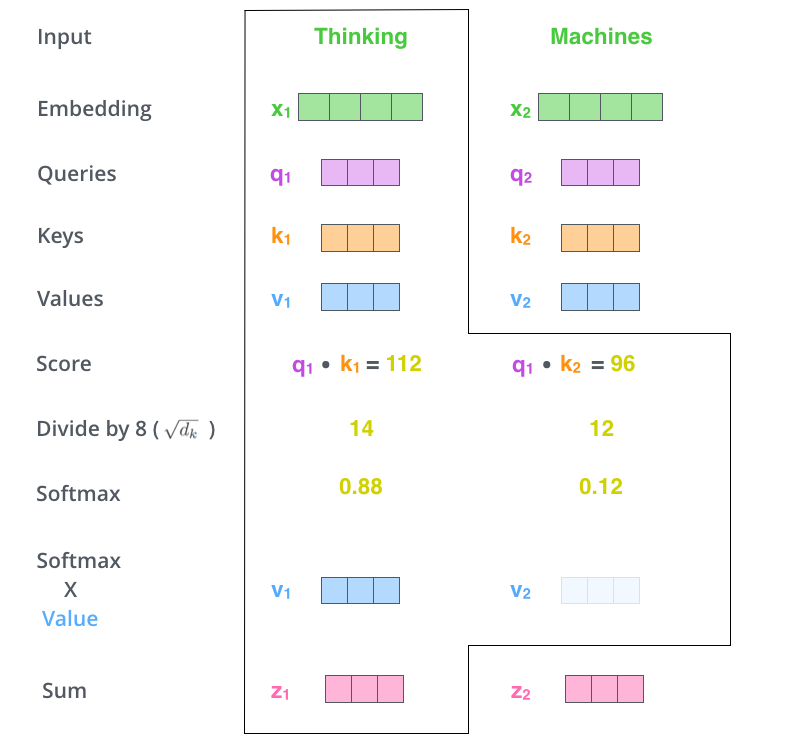
\includegraphics[scale = 0.3]{pics/self-attention-output.png}
        \end{figure} 


\end{frame}



\begin{frame}{Matrix Calculation of Self-Attention}
\begin{scriptsize}
\begin{itemize}

\item  In the actual implementation, scaled dot product self-attention is computed in matrix form for faster processing.
\item So let’s look at that now that we’ve seen the intuition of the calculation on the word level.

\item The first step is to calculate the Query, Key, and Value matrices: \textcolor{purple}{Q}, \textcolor{orange}{K}, \textcolor{blue}{V}.

\item We do that by packing our embeddings into a matrix $X$, and multiplying it by the weight matrices we’ve trained (\textcolor{purple}{WQ}, \textcolor{orange}{WK}, \textcolor{blue}{WV}).



 \begin{displaymath}
  \text{Attention}(Q,K,V) = \text{softmax}\left(\frac{QK^T}{\sqrt{d_k}}\right)*V
 \end{displaymath}





\end{itemize}

\end{scriptsize}

\end{frame}



\begin{frame}{Matrix Calculation of Self-Attention}

\begin{figure}[h]
        	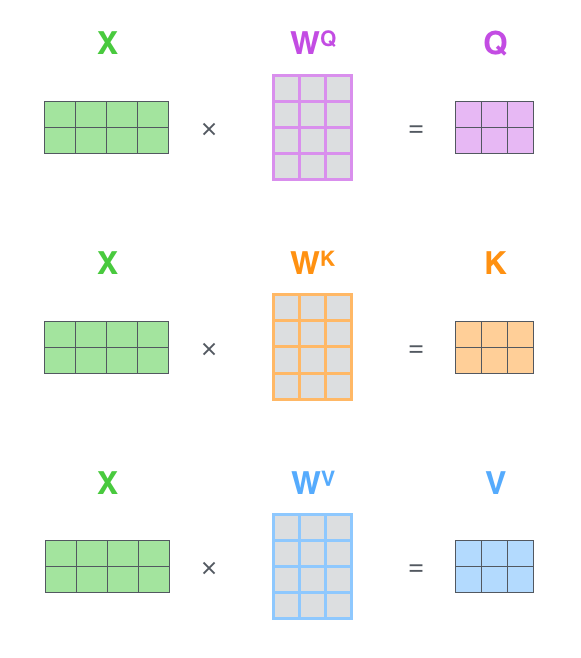
\includegraphics[scale = 0.25]{pics/self-attention-matrix-calculation.png}
        \end{figure} 

\begin{scriptsize}
\begin{itemize}

\item Every row in the X matrix corresponds to a word in the input sentence.
\item We again see the difference in size of the embedding vector (512, or 4 boxes in the figure), and the q/k/v vectors (64, or 3 boxes in the figure).


\end{itemize}

\end{scriptsize}

\end{frame}


\begin{frame}{Matrix Calculation of Self-Attention}



\begin{scriptsize}
\begin{itemize}

\item Finally, since we’re dealing with matrices, we can condense steps two through six in one formula to calculate the outputs of the self-attention layer.

\end{itemize}

\end{scriptsize}


\begin{figure}[h]
        	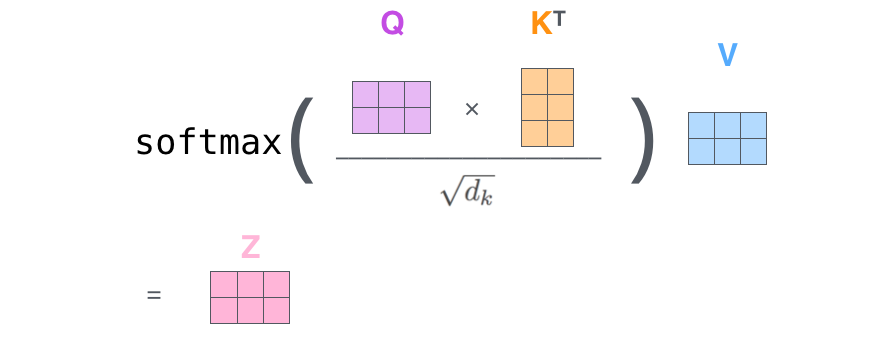
\includegraphics[scale = 0.35]{pics/self-attention-matrix-calculation-2.png}
        \end{figure} 

\end{frame}



\begin{frame}{Multi-Head Attention}
\begin{scriptsize}
\begin{itemize}

\item If we only compute a single attention weighted sum of the values, it would be difficult to capture various different aspects of the input.
\item In the example above, $z1$ contains a little bit of every other encoding, but it could be dominated by the actual word itself.
\item If we’re translating a sentence like ``The animal didn’t cross the street because it was too tired'', it would be useful to know which word ``it'' refers to.

\item To solve this problem, the Transformer uses the Multi-Head Attention block.
\item This component expands the model's ability to focus on different positions.
\item Multi-head attention computes multiple attention weighted sums instead of a single attention pass over the values.
\item Hence the name ``Multi-Head'' Attention.
\item To learn diverse representations, the Multi-Head Attention applies different linear transformations to the values, keys, and queries for each ``head'' of attention.
 
 
\end{itemize}

\end{scriptsize}

\end{frame}



\begin{frame}{Multi-Head Attention}
\begin{scriptsize}
\begin{itemize}
 \item The Multi-Head Attention block applies multiple blocks in parallel, concatenates their outputs, then applies one single linear transformation.
 
 
     \begin{figure}[h]
        	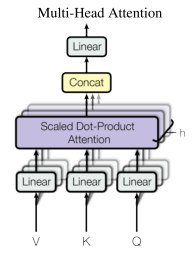
\includegraphics[scale = 0.48]{pics/multi_head_attention.png}
        \end{figure}  
 

\end{itemize}

\end{scriptsize}

\end{frame}






\begin{frame}{Multi-Head Attention}
\begin{scriptsize}


\begin{itemize}


\item The multi-headed component gives the attention layer multiple ``representation subspaces''.
\item With multi-headed attention, we have not only one, but multiple sets of Query/Key/Value weight matrices.
\item The Transformer uses eight attention heads, so we end up with eight sets for each encoder/decoder.
\item Each of these sets is randomly initialized.
\item Then, after training, each set is used to project the input embeddings (or vectors from lower encoders/decoders) into a different representation subspace.
 
\end{itemize}

\end{scriptsize}

\end{frame}



\begin{frame}{Multi-Head Attention}

     \begin{figure}[h]
        	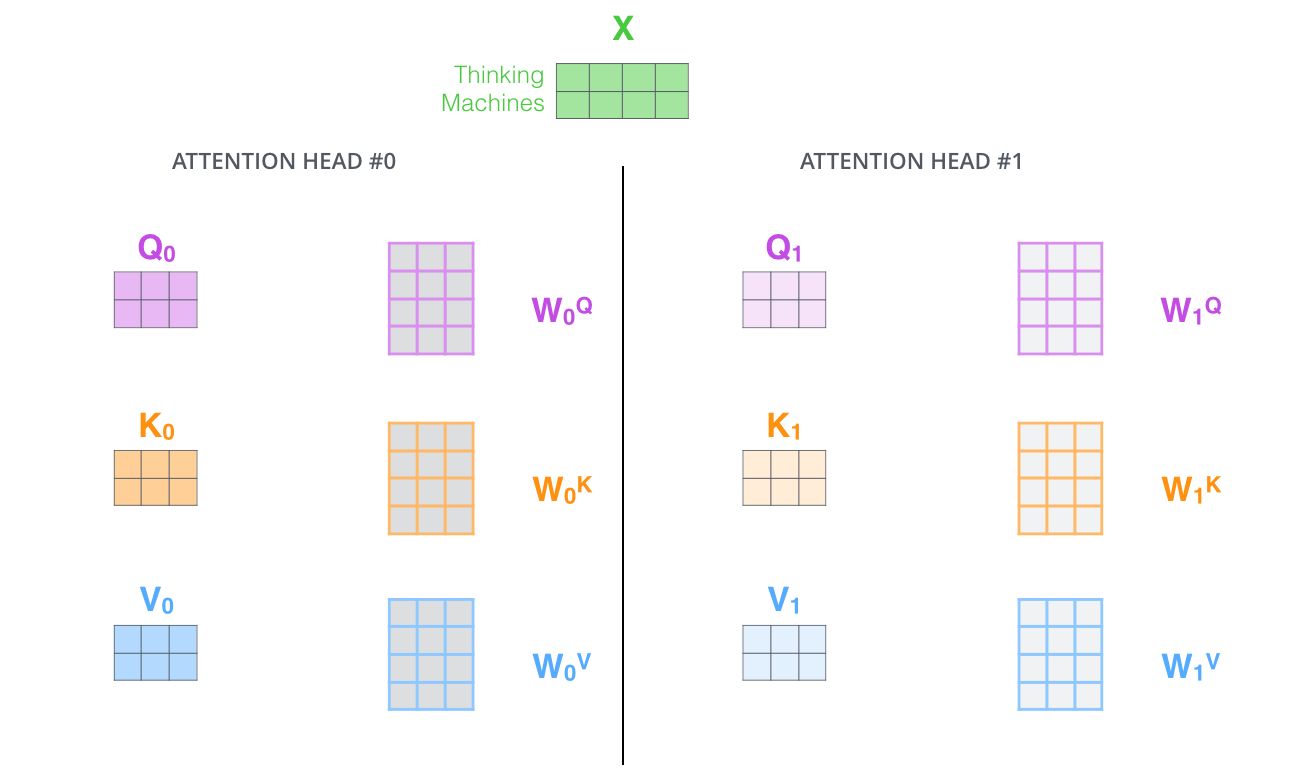
\includegraphics[scale = 0.2]{pics/transformer_attention_heads_qkv.png}
        \end{figure}


\begin{scriptsize}
\begin{itemize}
 \item With multi-headed attention, we maintain separate Q/K/V weight matrices for each head resulting in different Q/K/V matrices.
 \item As we did before, we multiply X by the WQ/WK/WV matrices to produce Q/K/V matrices.



\end{itemize}

\end{scriptsize}

\end{frame}


\begin{frame}{Multi-Head Attention}

     \begin{figure}[h]
        	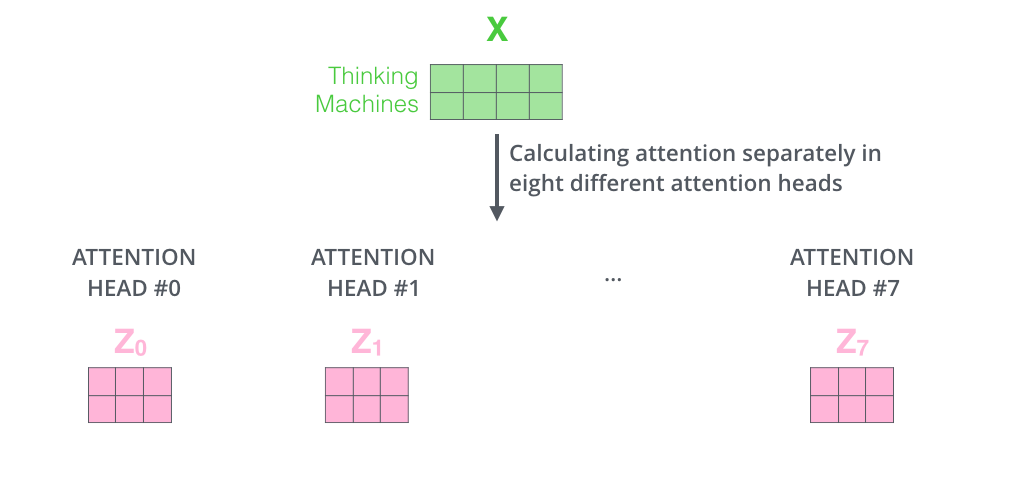
\includegraphics[scale = 0.25]{pics/transformer_attention_heads_z.png}
        \end{figure}


\begin{scriptsize}
\begin{itemize}
 \item If we do the same self-attention calculation we outlined above, just eight different times with different weight matrices, we end up with eight different Z matrices.
 \item This leaves us with a bit of a challenge.
 \item The feed-forward layer is not expecting eight matrices.
 \item It's expecting a single matrix (a vector for each word).
 \item So we need a way to condense these eight down into a single matrix.


\end{itemize}

\end{scriptsize}

\end{frame}



\begin{frame}{Multi-Head Attention}

\begin{scriptsize}
\begin{itemize}
 \item How do we do that? We concat the matrices then multiply them by an additional weights matrix WO.


\end{itemize}

\end{scriptsize}


     \begin{figure}[h]
        	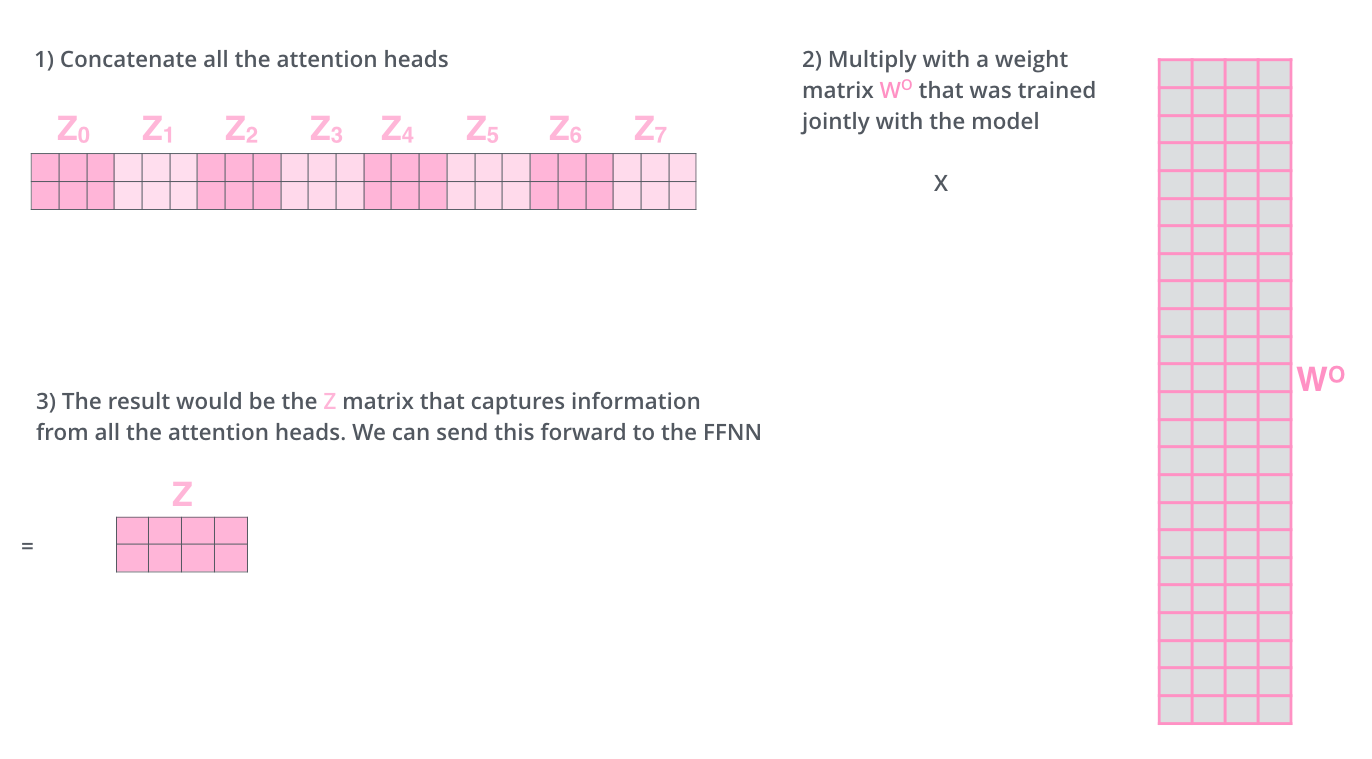
\includegraphics[scale = 0.22]{pics/transformer_attention_heads_weight_matrix_o.png}
        \end{figure}




\end{frame}


\begin{frame}{Multi-Head Attention}

\begin{scriptsize}
\begin{itemize}
 \item Let's put all these matrices in one visual so we can look at them in one place.


\end{itemize}

\end{scriptsize}


     \begin{figure}[h]
        	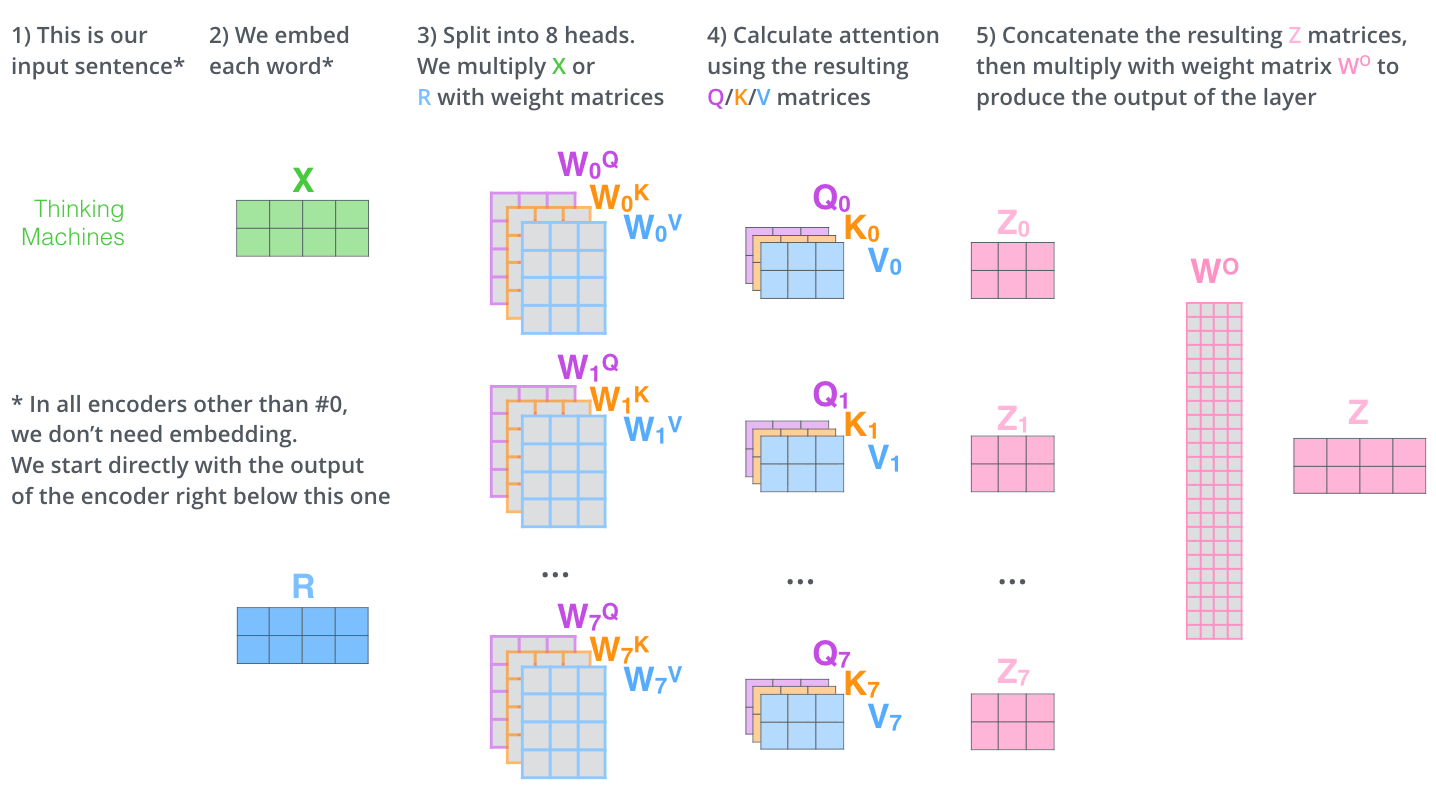
\includegraphics[scale = 0.226]{pics/transformer_multi-headed_self-attention-recap.png}
        \end{figure}




\end{frame}


\begin{frame}{Residual Connections}
\begin{scriptsize}
\begin{itemize}

\item Between each sub-layer, there is a residual connection followed by a layer normalization. 

\item A residual connection is basically just taking the input and adding it to the output of the sub-network, and is a way of making training deep networks easier. 

\item Layer normalization is a normalization method in deep learning that is similar to batch normalization.
 
\end{itemize}

\end{scriptsize}


 \begin{figure}[h]
        	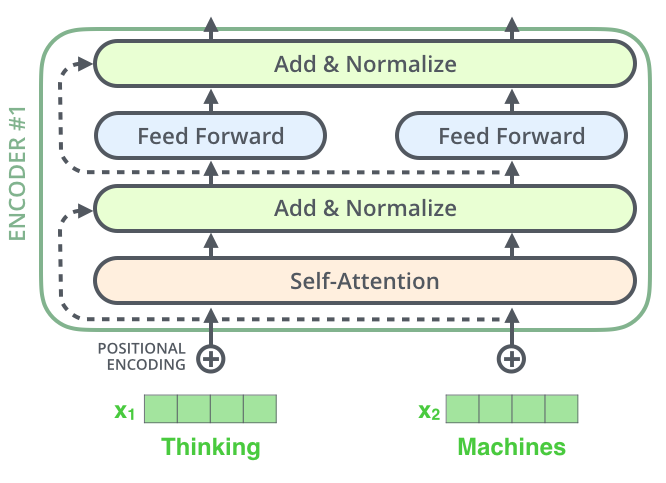
\includegraphics[scale = 0.3]{pics/transformer_resideual_layer_norm.png}
        \end{figure}


\end{frame}

\begin{frame}{Residual Connections}
\begin{scriptsize}
\begin{itemize}

\item If we’re to visualize the vectors and the layer-norm operation associated with self attention, it would look like this:

\end{itemize}

\end{scriptsize}


 \begin{figure}[h]
        	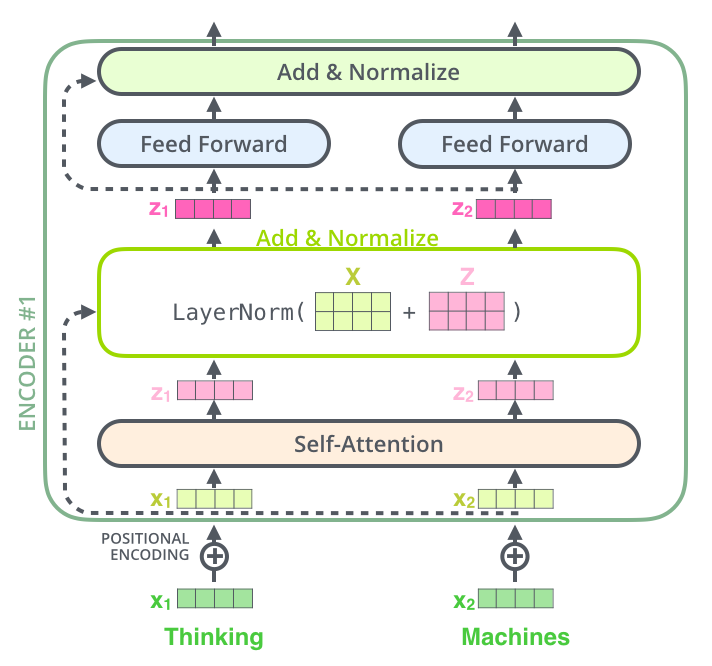
\includegraphics[scale = 0.3]{pics/transformer_resideual_layer_norm_2.png}
        \end{figure}


\end{frame}



\begin{frame}{The Encoder: summary}

     \begin{figure}[h]
        	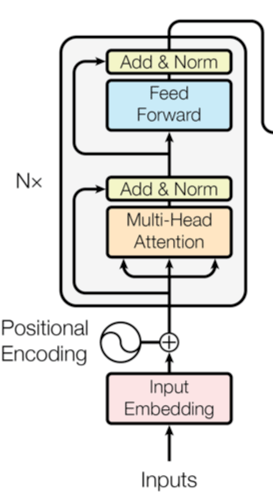
\includegraphics[scale = 0.39]{pics/transformerencoder.png}
        \end{figure}  


\end{frame}

\begin{frame}{The Encoder: summary}
\begin{scriptsize}
\begin{itemize}

 \item  What each encoder block is doing is actually just a bunch of matrix multiplications followed by a couple of element-wise transformations.

 \item This is why the Transformer is so fast: everything is just parallelizable matrix multiplications.

 \item The point is that by stacking these transformations on top of each other, we can create a very powerful network.

 \item The core of this is the attention mechanism which modifies and attends over a wide range of information.

\end{itemize}

\end{scriptsize}

\end{frame}



\begin{frame}{The Decoder}
\begin{scriptsize}
\begin{itemize}

\item The Transformer decoder utilizes the output of the top encoder to generate attention vectors K and V. 
\item These attention vectors are then employed by each decoder in its ``encoder-decoder attention'' layer to enable the decoder to focus on relevant sections in the input sequence.

\item By doing so, every position in the decoder is able to attend to all positions in the input sequence, replicating the typical encoder-decoder attention mechanisms found in sequence-to-sequence models. 

\item Additionally, self-attention layers within the decoder allow each position to attend to all positions within the decoder, including itself, similar to the role played by the decoder hidden state in RNN machine translation architectures.

\item In summary, the ``Encoder-Decoder Attention`` layer works just like multiheaded self-attention, except it creates its Queries matrix from the layer below it, and takes the Keys and Values matrix from the output of the encoder stack.


 
\end{itemize}

\end{scriptsize}

\end{frame}


\begin{frame}{The Decoder}

     \begin{figure}[h]
        	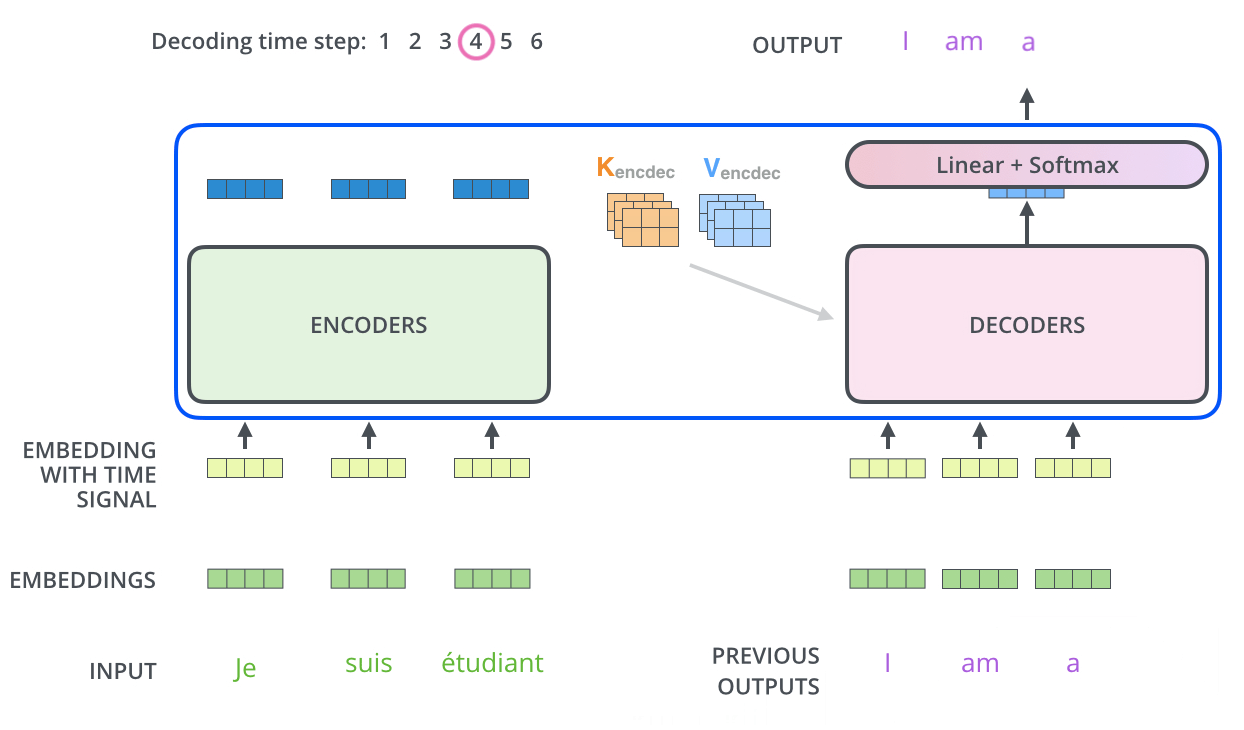
\includegraphics[scale = 0.28]{pics/transformer_decoder.png}
        \end{figure}  

\begin{scriptsize}
\begin{itemize}

 \item Each step in the decoding phase outputs an element from the output sequence (the English translation sentence in this case). 
 \item This process is repeated until a special symbol is reached indicating the transformer decoder has completed its output.
\end{itemize}

\end{scriptsize}
        
        
\end{frame}



\begin{frame}{The Decoder}
\begin{scriptsize}
\begin{itemize}
 \item When we train the Transformer, we want to process all the sentences at the same time. 
 
 \item However, if we give the decoder access to the entire target sentence, the model can just repeat the target sentence (in other words, it doesn't need to learn anything).
 
 \item The self-attention layer should only be allowed to attend to earlier positions in the output sequence.
 
 \item This is done by masking the ``future'' tokens when decoding a certain word.

  \item The masking is done by setting to $- \infty$ all values in the input of the softmax which correspond to illegal connections.
 \item This is why ``multi-head attention blocks'' in the decoder are referred to as ``masked'': the inputs to the decoder from future time-steps are masked.
 
 
\end{itemize}

\end{scriptsize}

\end{frame}


\begin{frame}{The Decoder}

     \begin{figure}[h]
        	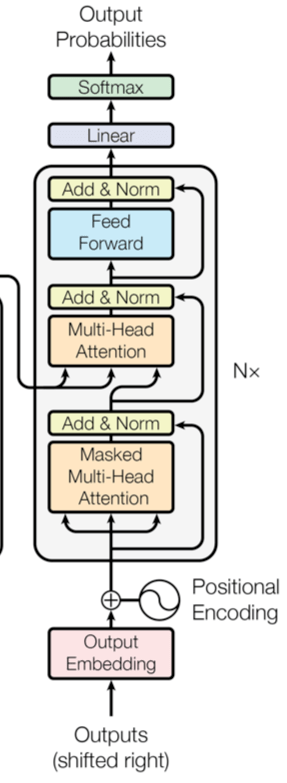
\includegraphics[scale = 0.29]{pics/transformerdecoder.png}
        \end{figure}  


\end{frame}



\begin{frame}{Positional Encodings}
\begin{scriptsize}
\begin{itemize}

 \item  Unlike recurrent networks, the multi-head attention network cannot naturally make use of the position of the words in the input sequence.
 
 \item Without positional encodings, the output of the multi-head attention network would be the same for the sentences ``I like cats more than dogs'' and ``I like dogs more than cats''.
 
 \item Positional encodings explicitly encode the relative/absolute positions of the inputs as vectors and are then added to the input embeddings.

\end{itemize}

\end{scriptsize}


\end{frame}

\begin{frame}{Positional Encodings}


   \begin{figure}[h]
        	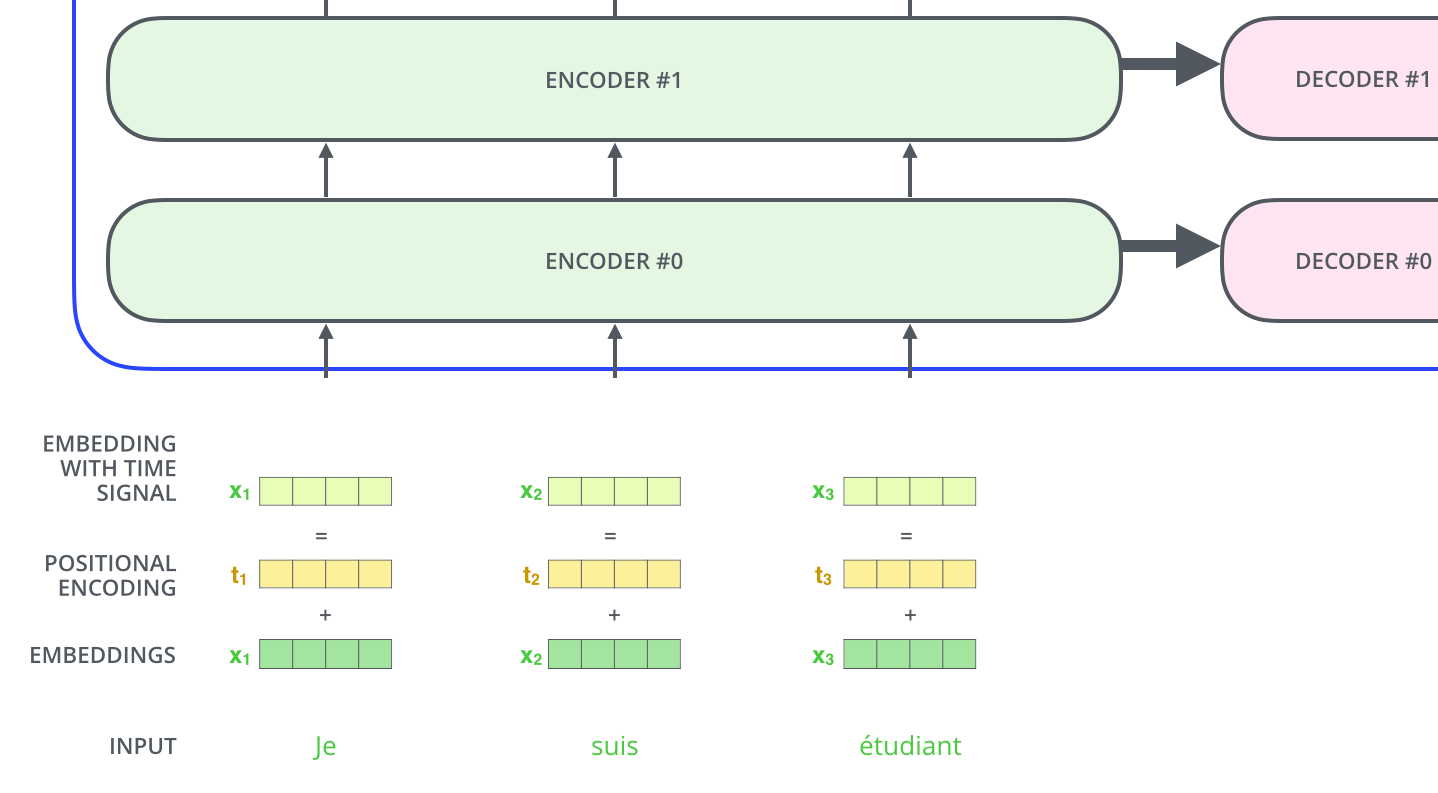
\includegraphics[scale = 0.2]{pics/transformer_positional_encoding_vectors.png}
        \end{figure}  




\begin{scriptsize}
\begin{itemize}

 \item To give the model a sense of the order of the words, we add positional encoding vectors -- the values of which follow a specific pattern. 


\end{itemize}

\end{scriptsize}


\end{frame}


\begin{frame}{Positional Encodings}
\begin{scriptsize}
\begin{itemize}

 \item The paper uses the following equation to compute the positional encodings: \\
 $PE(pos,2i) = \sin(pos/10000^{2i/d_{model}})$ 
  $PE(pos,2i+1) = \cos(pos/10000^{2i/d_{model}})$
 
\item Where $pos$ represents the position, and $i$ is the dimension.

\item Basically, each dimension of the positional encoding is a wave with a different frequency. 


   \begin{figure}[h]
        	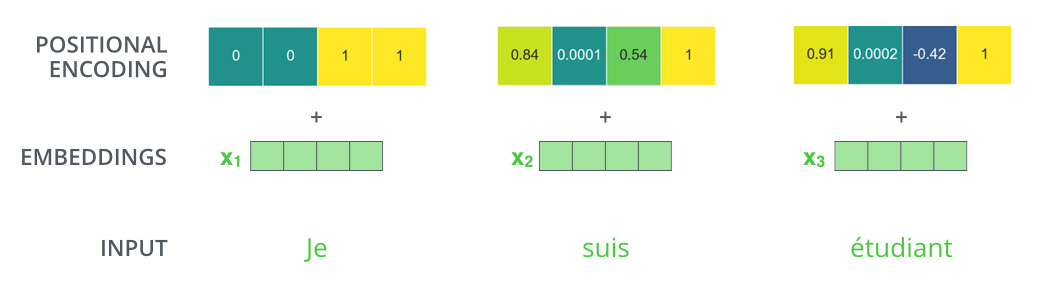
\includegraphics[scale = 0.25]{pics/transformer_positional_encoding_example.png}
        \end{figure}  



\item A real example of positional encoding with a toy embedding size of 4.



\end{itemize}

\end{scriptsize}


\end{frame}





\begin{frame}{Conclusions}
\begin{scriptsize}
\begin{itemize}

 \item The Transformer achieves better BLUE scores than previous state-of-the-art models for English-to-German translation and English-to-French translation at a fraction of the training cost.

      \begin{figure}[h]
        	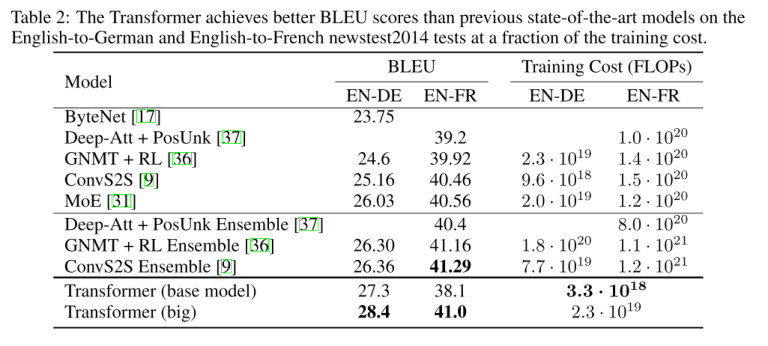
\includegraphics[scale = 0.29]{pics/transformerresults.png}
        \end{figure}  

\item The Transformer is a powerful and efficient alternative to recurrent neural networks to model dependencies using only attention mechanisms.

\item A very illustrative blog post about the Transformer: \url{http://jalammar.github.io/illustrated-transformer/}.
 
\end{itemize}

\end{scriptsize}


\end{frame}

\begin{frame}
\frametitle{Questions?}
%\vspace{1.5cm}
\begin{center}\LARGE Thanks for your Attention!\\ \end{center}



\end{frame}

\begin{frame}[allowframebreaks]\scriptsize
\frametitle{References}
\bibliography{bio}
\bibliographystyle{apalike}
%\bibliographystyle{flexbib}
\end{frame}  


%%%%%%%%%%%%%%%%%%%%%%%%%%%

\end{document}
